\documentclass[10pt]{beamer}

\mode<presentation> {

% \usetheme{Berlin}  % Squares
\usetheme{Madrid}  % Circles & dense
% \usetheme{Frankfurt}  % Cirles

\setbeamertemplate{headline}{%
\leavevmode%
  \hbox{%
    \begin{beamercolorbox}[wd=\paperwidth,ht=2.5ex,dp=1.125ex]{palette quaternary}%
    \insertsectionnavigationhorizontal{\paperwidth}{}{\hskip0pt plus1filll}
    \end{beamercolorbox}%
  }
}

\setbeamertemplate{navigation symbols}{}  % To remove the navigation symbols from the bottom of all slides uncomment this line

% \useoutertheme{miniframes}
% \useinnertheme{circles}

}

\usepackage{graphicx}
\usepackage{booktabs}
\usepackage{fontspec}
\usepackage{xunicode}
\usepackage{xltxtra}
\usepackage{xecyr}
\usepackage{hyperref}
\usepackage{amsthm}

\usepackage{polyglossia}
\setdefaultlanguage{russian}
\setmainfont[Mapping=tex-text]{CMU Serif}
\setsansfont[Mapping=tex-text]{CMU Sans Serif}
\setmonofont[Mapping=tex-text]{CMU Serif}
%-------------------------------------------------------------------------------
%	TITLE PAGE
%-------------------------------------------------------------------------------
\title[Controllable text generation]{Controllable text generation with small data using auxiliary in-domain enrichment}
\author{Беляев Станислав}
\institute[СПбАУ]
{
Санкт-Петербургский Академический Университет \\
\medskip
\textit{stasbelyaev96@gmail.com}
}
\date{23 марта 2018}

\begin{document}
%-------------------------------------------------------------------------------
%	PRESENTATION SLIDES
%-------------------------------------------------------------------------------
\begin{frame}
\titlepage
\end{frame}
%-------------------------------------------------------------------------------
\section{Введение}
\begin{frame}
\frametitle{Введение}
\framesubtitle{Обзор}

\begin{exampleblock}{}
  {\Large “If a typical person can do a mental task with less than one second of thought, we can probably automate it using AI either now or in the near future.”}
  \vskip2mm
  \hspace*\fill{\small--- Andrew Ng, 2017}
\end{exampleblock}

Машины умеют:
\begin{enumerate}
    \item Различать формы и объекты
    \item Имитировать стиль изображений
    \item Отвечать на простые вопросы
\end{enumerate}

Машины НЕ умеют:
\begin{enumerate}
    \item \underline{Хорошо} подражать высшей нервной деятельности
    \item Понимать и обощать сложные категории
    \begin{itemize}
        \item Этика (юмор, мораль, норма, ...)
        \item Эстетика (книги, картины, ...)
    \end{itemize}
\end{enumerate}

\end{frame}
%-------------------------------------------------------------------------------
\begin{frame}
\frametitle{Введение}
\framesubtitle{Постановка задачи}

\begin{columns}
    \begin{column}{0.7\textwidth}
        MOOC платформам нужна генерация контента:
        \begin{itemize}
            \item Дешево
            \item Быстро
            \item Ультимативная защита от списывания
        \end{itemize}
        
        Особенности:
        \begin{itemize}
            \item Generic характер генерации
            \item Примеров готового контента мало
            \item Набор текстовых свойств для единицы контента (курс, тема, тэги, сложность, ...)
        \end{itemize}
    \end{column}
    \begin{column}{0.3\textwidth}
        \begin{center}
            
\includegraphics[height=3.5cm]{images/stepik.png}
        \end{center}
    \end{column}
\end{columns}

\vskip4mm

\underline{Задача}: По набору свойств $f = \{f_i \in F\}$ сгенерировать новые примеры текстовых данных из генеральной совокупности $X$, соответствующих $f$. \\
Возьмем в качестве $X$ условия задачек по программированию.

\end{frame}
%-------------------------------------------------------------------------------
\begin{frame}
\frametitle{Введение}
\framesubtitle{Данные в DL}

\begin{exampleblock}{}
  {\large “Data is the New Oil.”}
  \vskip1mm
  \hspace*\fill{\small--- Andrew Ng, 2017}
\end{exampleblock}

\begin{columns}
    \begin{column}{0.5\textwidth}
        \begin{center}
            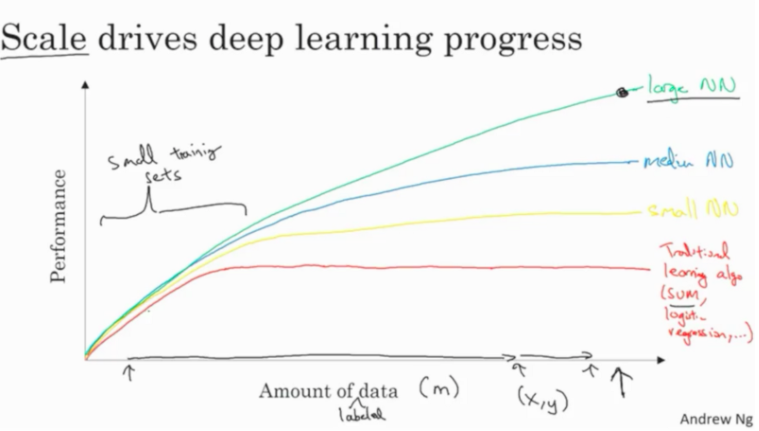
\includegraphics[width=\textwidth]{images/dl_tradeoff.png}
        \end{center}
    \end{column}
    \vline
    \begin{column}{0.5\textwidth}
        \begin{center}
            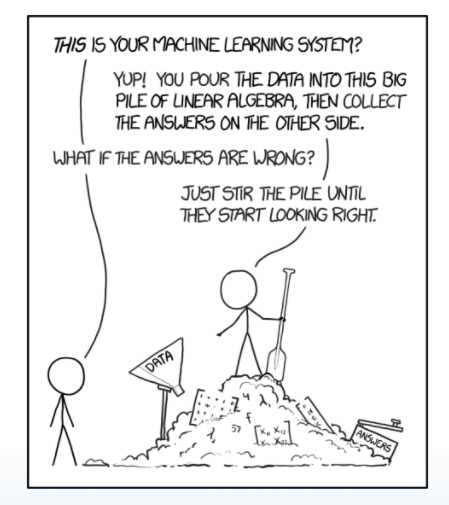
\includegraphics[height=5.5cm]{images/dl_data_joke.png}
        \end{center}
    \end{column}
\end{columns}

\end{frame}
%-------------------------------------------------------------------------------
\begin{frame}
\frametitle{Введение}
\framesubtitle{Проблема данных}

Если мы не знаем паттерна для генерации и хотим уметь обощать, то будем использовать DL и больше данных (Mikolov et al., 2010). \\

\begin{columns}
    \begin{column}{0.5\textwidth}
        Но что делать, есть данных мало?
        \begin{itemize}
            \item Мы не сможем обобщать 
            \item Мы скорее всего переобучимся
            \item При генерации новые сэмплы будут слишком похожи на старые
        \end{itemize}
    \end{column}
    \begin{column}{0.5\textwidth}
        \begin{center}
            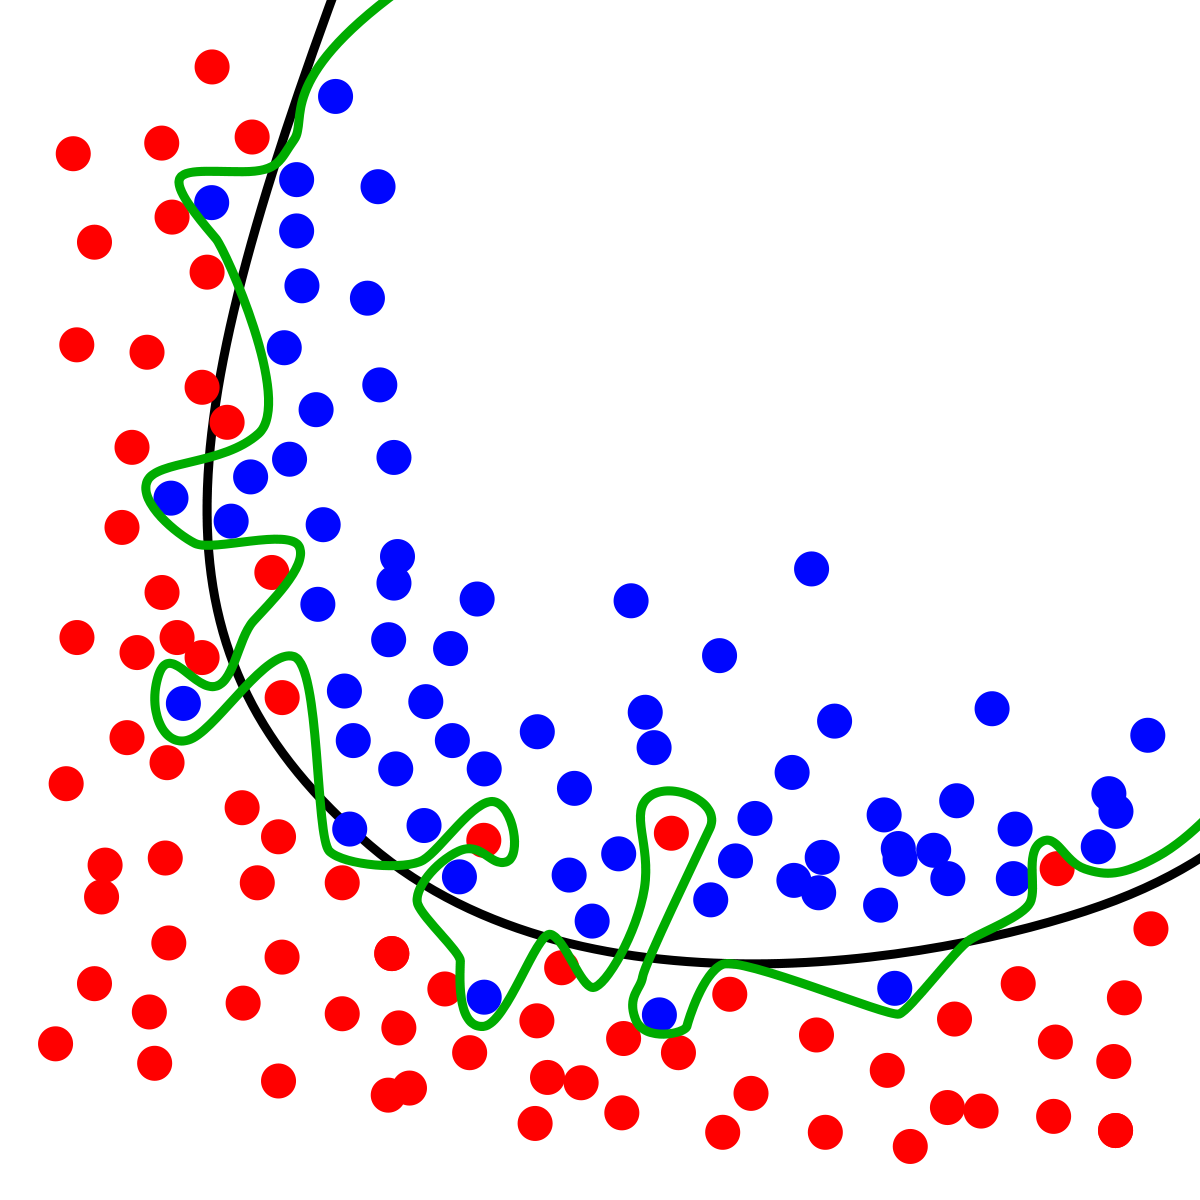
\includegraphics[width=0.7\textwidth]{images/overfitting.png}
        \end{center}
    \end{column}
\end{columns}

\vskip4mm

\underline{Решение}: Искать похожие $X_{aux} \sim X$ in-domain данные из смежных областей.

\end{frame}
%-------------------------------------------------------------------------------
\begin{frame}
\frametitle{Введение}
\framesubtitle{Изображения vs текст}

\begin{columns}[T]
    \begin{column}[T]{0.5\textwidth}
        \begin{center}
            Изображения \\
            
\includegraphics[width=0.5\textwidth]{images/image_as_func.png} \\
            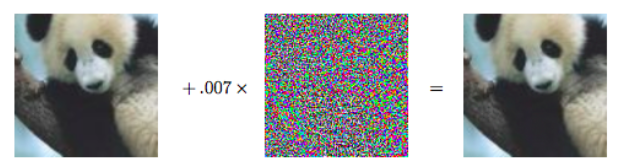
\includegraphics[width=\textwidth]{images/panda_plus_noise.png} \\
            \begin{itemize}
                \item Непрерывное пространство
                \item Набор всевозможных преобразований как дифференцируемых функций
                \item Понятно, куда распространять градиент
            \end{itemize}
        \end{center}
    \end{column}
    \vline
    \begin{column}[T]{0.5\textwidth}
        \begin{center}
            Текст \\
            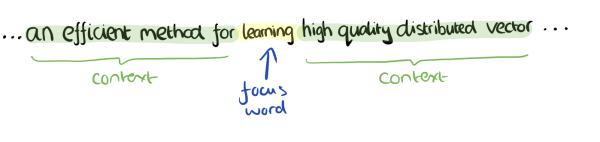
\includegraphics[width=0.9\textwidth]{images/word_context.png} \\
            \begin{itemize}
                \item Дискретное пространство
                \item Переменная длинна
                \item Нет устойчивости к шуму
                \item Long-term зависимости
                \item Омонимия и контекст
            \end{itemize}
        \end{center}
    \end{column}
\end{columns}

\end{frame}
%-------------------------------------------------------------------------------
\begin{frame}
\frametitle{Введение}
\framesubtitle{Генерация текста}

\begin{columns}[T]
    \begin{column}[T]{0.33\textwidth}
        \begin{center}
            RNN \\
            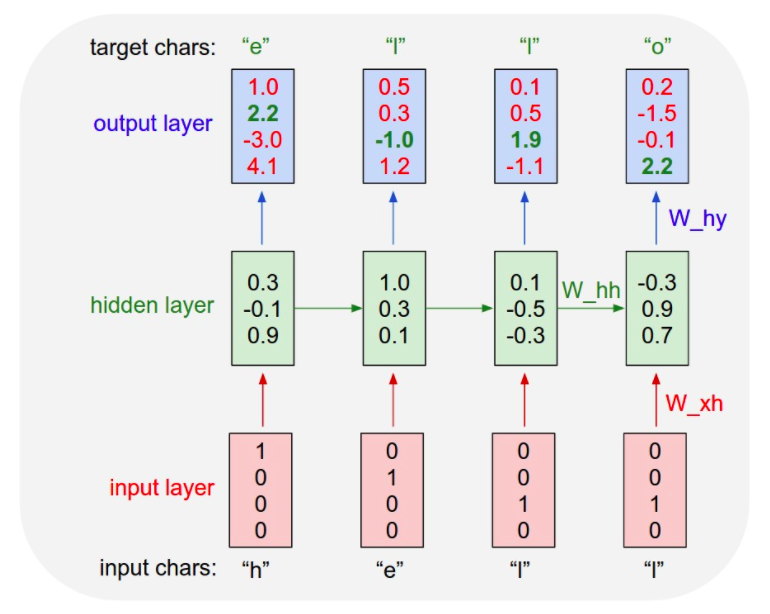
\includegraphics[width=\textwidth]{images/rnn.png} \\
            (Mikolov et al., 2011)
        \end{center}
    \end{column}
    \vline
    \begin{column}[T]{0.33\textwidth}
        \begin{center}
            VAE \\
            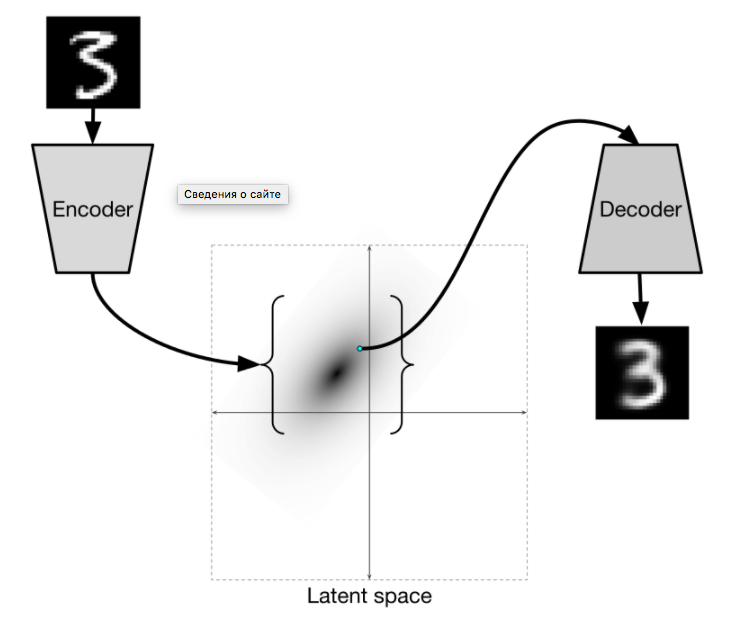
\includegraphics[width=0.9\textwidth]{images/vae.png} \\
            (Bowman et al., 2016; Hu et al., 2018)
        \end{center}
    \end{column}
    \vline
    \begin{column}[T]{0.33\textwidth}
        \begin{center}
            GAN \\
            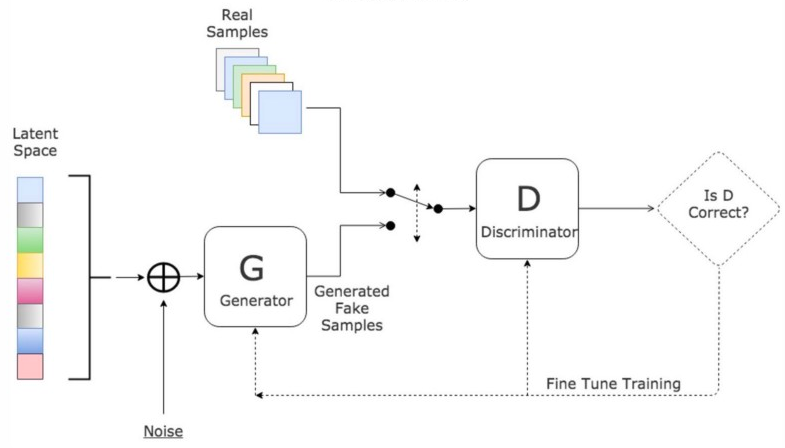
\includegraphics[width=0.9\textwidth]{images/gan.png} \\
            (Yu et al., 2017; Fedus et al., 2018)
        \end{center}
    \end{column}
\end{columns}

\end{frame}
%-------------------------------------------------------------------------------
\section{Данные}
\begin{frame}
\frametitle{Данные}
\framesubtitle{Источники}

Разберемся, откуда брать данные...

\end{frame}
%-------------------------------------------------------------------------------
\section{RNN}
\begin{frame}
\frametitle{RNN}
\framesubtitle{Обзор}

RNN

\end{frame}
%-------------------------------------------------------------------------------
\section{VAE}
\begin{frame}
\frametitle{VAE}
\framesubtitle{Обзор}

VAE

\end{frame}
%-------------------------------------------------------------------------------
\section{GAN}
\begin{frame}
\frametitle{GAN}
\framesubtitle{Обзор}

GAN

\end{frame}
%-------------------------------------------------------------------------------
\section{Оценивание}
\begin{frame}
\frametitle{Оценивание}
\framesubtitle{Метрики}

Perplexity и смотреть глазками \\

\begin{table}
\begin{tabular}{l l l}
\toprule
\textbf{Treatments} & \textbf{Response 1} & \textbf{Response 2}\\
\midrule
Treatment 1 & 0.0003262 & 0.562 \\
Treatment 2 & 0.0015681 & 0.910 \\
Treatment 3 & 0.0009271 & 0.296 \\
\bottomrule
\end{tabular}
\caption{Table caption}
\end{table}

\end{frame}
%-------------------------------------------------------------------------------
\section{Выводы}
\begin{frame}
\frametitle{Выводы}
\framesubtitle{Результаты}

То то и то то

\end{frame}
%-------------------------------------------------------------------------------
\section{Ссылки}
\begin{frame}
\frametitle{Ссылки}
\framesubtitle{Статьи}

То то и то то \\

\footnotesize{
\begin{thebibliography}{99}
\bibitem[Smith, 2012]{p1} John Smith (2012)
\newblock Title of the publication
\newblock \emph{Journal Name} 12(3), 45 -- 678.
\end{thebibliography}
}

\end{frame}
%-------------------------------------------------------------------------------
%	END PRESENTATION SLIDES
%-------------------------------------------------------------------------------
\end{document}